\documentclass[12pt]{article}

\usepackage{amsmath}
\usepackage[margin=0.75in]{geometry}
\usepackage[numbers]{natbib}
\usepackage{physics}
\usepackage[hyphens]{url}
\usepackage[labelformat=simple,position=b]{subcaption}
\renewcommand\thesubfigure{(\alph{subfigure})}
\usepackage{fancyhdr}
\pagestyle{fancy}
\fancyhf{}
\rhead{Team 10}
\lhead{Week 1: Trapped ions}
\rfoot{Page \thepage}

\usepackage{graphicx}
\graphicspath{
	{figures}
}

\usepackage[hidelinks]{hyperref}


\renewcommand{\phi}{\varphi}


\title{Week 1: Simulating quantum advantage with trapped ions}
\author{Team 10: Alexander (Sandy) Bell, 
\and Na Young Kim, 
\and Sushanta Mitra, 
\and Ushnish Ray, 
\and Ming-Tso Wei}
\date{\today}


\begin{document}

\maketitle

%\thispagestyle{empty}


\section*{Introduction}

We put all the functions for the coding tasks in the script \texttt{assignment.jl}.

%% Ray: do you need to explain some of your code about the modification of "run" function, like the use of MersenneTwister.


\section*{Task 1}
In this task, we create a function \texttt{getAmp2} to calculate the probability $P(x)= \abs{\ip{x}{\psi}}^2$ of each bit-string $x$ by taking a dot product between the the MPS ($|\psi\rangle$) and a simple product state $|x\rangle$
(of bond dimension $D = 1$). The state $|\psi\rangle$ is obtained by applying the quantum circuit made of random one qubit and two qubit gates applied to the $N$ qubits of the system we are simulating. These gates are applied in layers leading to an effective circuit of depth $d$. In Fig. \ref{fig:speckle}, we plot 16 speckle patterns representing the state for a system of $N \in \{2,3,4,5\}$ qubits and random quantum circuits of depth $d \in \{ 4, 16, 32, 64\}$. Each speckle pattern consists of red circles with an area proportional to the probability. Owing to the random nature of the circuit one finds that the probabilities associated with different states are distributed randomly.

\begin{figure}[!b]
	\centering
	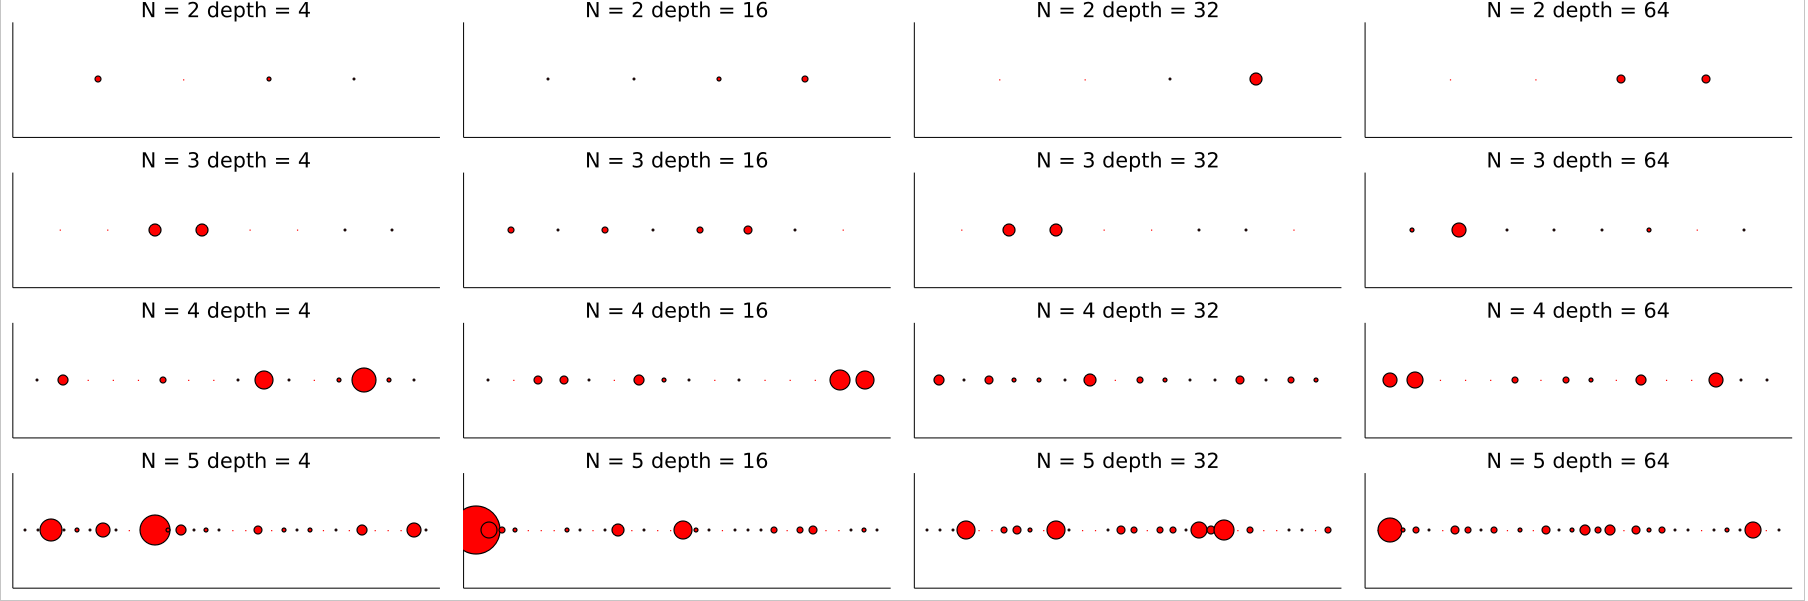
\includegraphics [width=\linewidth] {figures/Task_1a}
	\caption{
		``Speckle patterns'' displaying the probabilities of obtaining with $N=2$ to 5 and depths of 4, 16, 32, and 64.
	}
	\label{fig:speckle}
\end{figure}

We also make a function \texttt{studyBondDim} to calculate the bond dimension in the bonus problem by using the built-in function \texttt{maxlinkdim} in ITensor. In Fig. \ref{fig:bonddim}, we plot the bond dimensions as a function of circuit depth at several values of $N$. In all cases the function returns the bond dimension associated with the central link of the MPS. It is straightforward to see that as the circuit depth is increase the entanglement in the system grows and ultimately saturates at the largest possible value $2^{N/2}$, i.e., $D = 2, 4, 8, 16, 32, 64$ for $N = 2, 4, 6, 8, 10 ,12$. Note that as the circuits are random the scaling can be noisy. As such we perform an average over 20 random circuits to get a better understanding of the scaling. 

\begin{figure}[t]
	\centering
	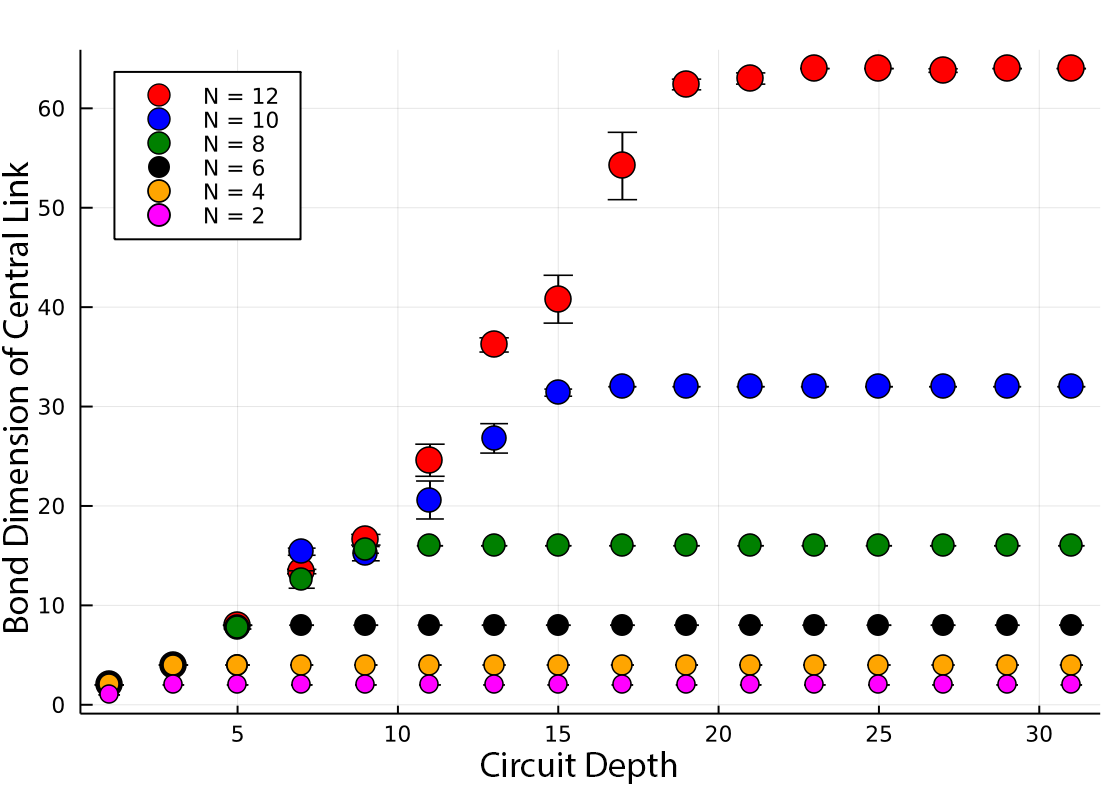
\includegraphics [width=0.8\linewidth] {figures/Task1b}
	\caption{
		The bond dimensions of the central link associated with the MPS as a function of circuit depth for varying number of qubits.}
	\label{fig:bonddim}
\end{figure}


\section*{Task 2}

To consider a single random bit flip, we modified the given \texttt{run} function by adding an argument \texttt{wbitflip}. If \texttt{wbitflip} is \texttt{True}, we assign a bit flip operator ($\hat{\sigma}_z$) at a random location (layer and qubit) of the circuit. In Fig. \ref{fig:bitflip}, we plot 16 different speckle patterns that result from the bit flip error.

\begin{figure}[th]
	\centering
	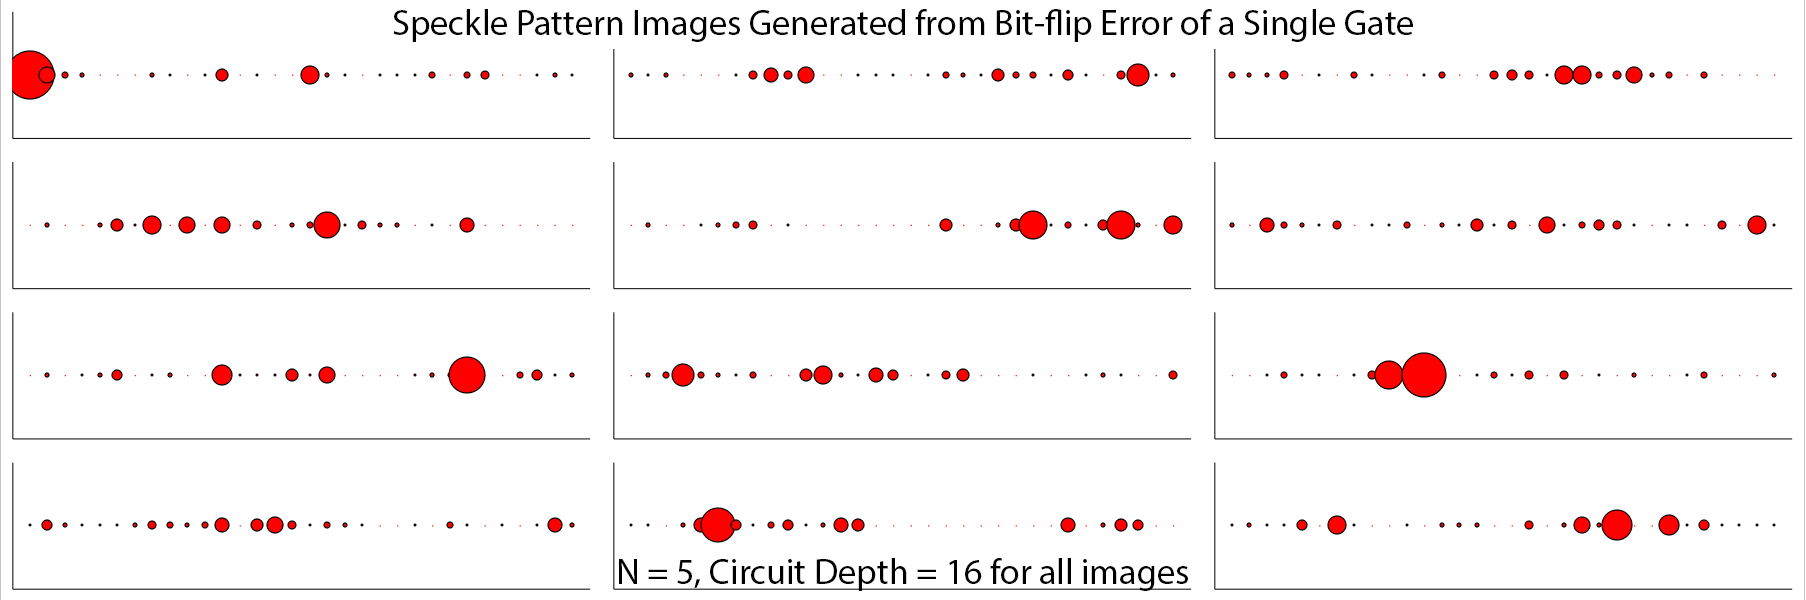
\includegraphics [width=\linewidth] {figures/Task2}
	\caption{
		 ``Speckle patterns'' displaying the probabilities of obtaining each of the 16 possible outcomes when sampling a 5-qubit circuit with a bit flip error occurred at a random location.
	}
	\label{fig:bitflip}
\end{figure}

\section*{Task 3}

In this task, we create a function \texttt{cgfScalingSingle} to calculate the cumulative distribution function (CDF) by numerically summing or integrating the probability distribution. Then we use the function \texttt{cgfScaling} to plot the CDF values with different depths and compare them with the theoretical value $1-e^{-2^Np}$, as shown in Fig. \ref{fig:cdf}

\begin{figure}[t]
	\centering
	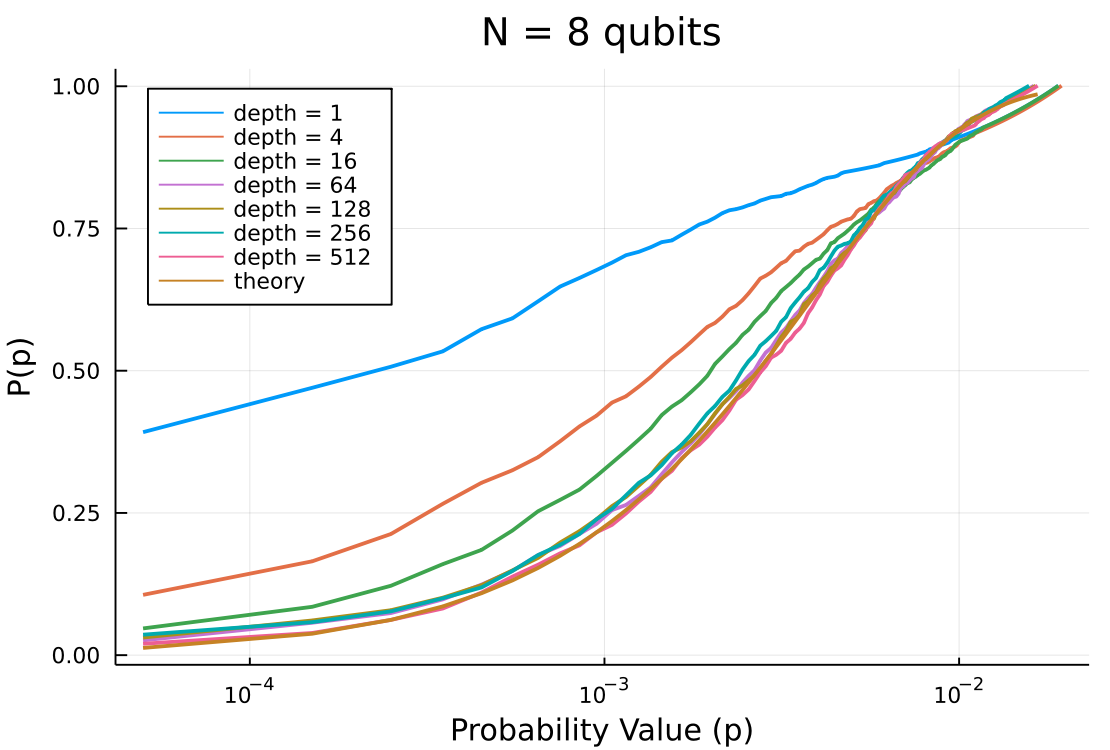
\includegraphics [width=0.8\linewidth] {figures/Task3}
	\caption{
		Calculated CDF as a function of the probability values $p$ in log scale at different circuit depths in an 8-qubit circuit. When the depth is larger, the CDF converges toward the theoretical value $1- e^{-2^Np}$. These were calculate using 1000 samples and a mesh size of $dp = 0.0001$ for binning.
	}
	\label{fig:cdf}
\end{figure}

\section*{Task 4}
In the function \texttt{crossEntropyValue}, we calculate the linear cross-entropy benchmarking (XEB) fidelity $\mathcal{F}_\mathrm{XEB}$ between two states $|\psi_0\rangle$ and $|\psi_1\rangle$ as $\mathcal{F}_\mathrm{XEB} = 2^N \sum_{x} |\langle x|\psi_0\rangle|^2 |\langle x|\psi_1\rangle|^2 - 1$. This is used as a helper function for computations of interest in this task. 

In Fig. \ref{fig:task4}, the function \texttt{crossEntropy} computes $\mathcal{F}_\mathrm{XEB} = 2^N \sum_{x} |\langle x|\psi_0\rangle|^2 |\langle x|\psi_0(\Delta\Theta) \rangle|^2 - 1$, i.e. the linear cross-entropy benchmarking (XEB) fidelity between the static state $|\psi_0\rangle$ generated from a single random circuit and $\psi_0(\Delta \Theta)\rangle$ generated by perturbing every 2-qubit gate of the static circuit by an angle $\Delta \Theta$. This results is for a system of $N = 8$ qubits and circuit depth of $d = 512$. The lack of averaging over random samples makes it difficult to understand the behaviour of the function leading to negative numbers in some cases (this is particularly true for small depths and system sizes). Consequently in in Figs. \ref{fig:XEBfidelity} (b) - (d), we calculate $\mathcal{F}_\mathrm{XEB}$ by averaging over a number of samples. This allows us to see a remarkable resurgence of $\mathcal{F}_\mathrm{XEB}$ at $\Delta \Theta = \pi$.

\begin{figure}[t]
	\centering
	\begin{subfigure}[t]{0.42\textwidth}
		\centering
		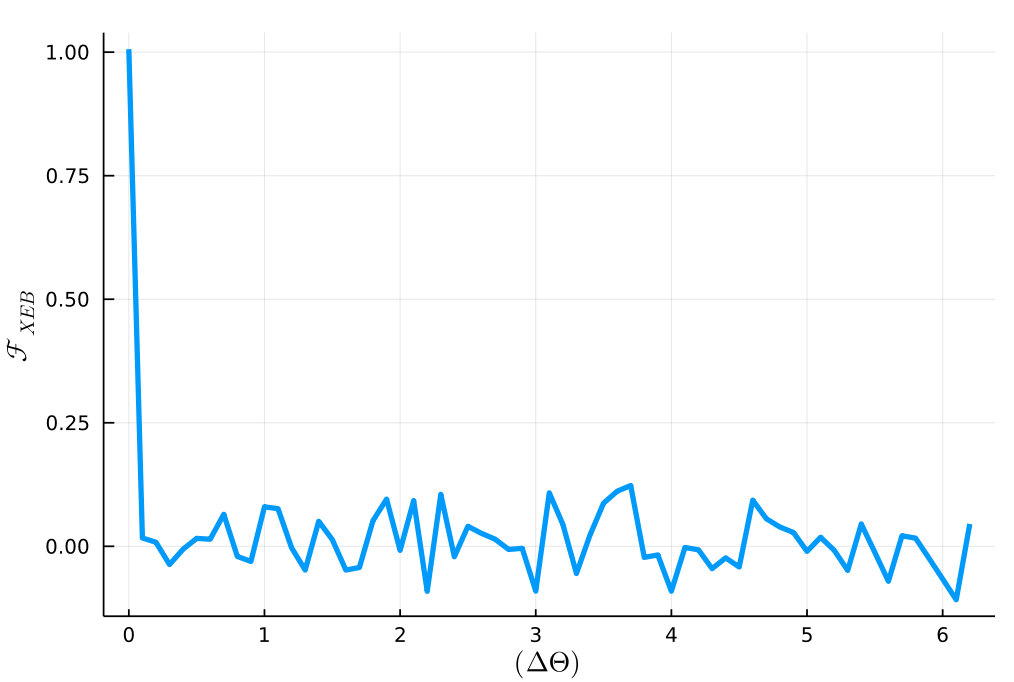
\includegraphics[width=\linewidth]
		{figures/Task4_N_8_d_512_s_1}
		\subcaption{\label{fig:task4}}
	\end{subfigure}%a
	\begin{subfigure}[t]{0.42\textwidth}
		\centering
		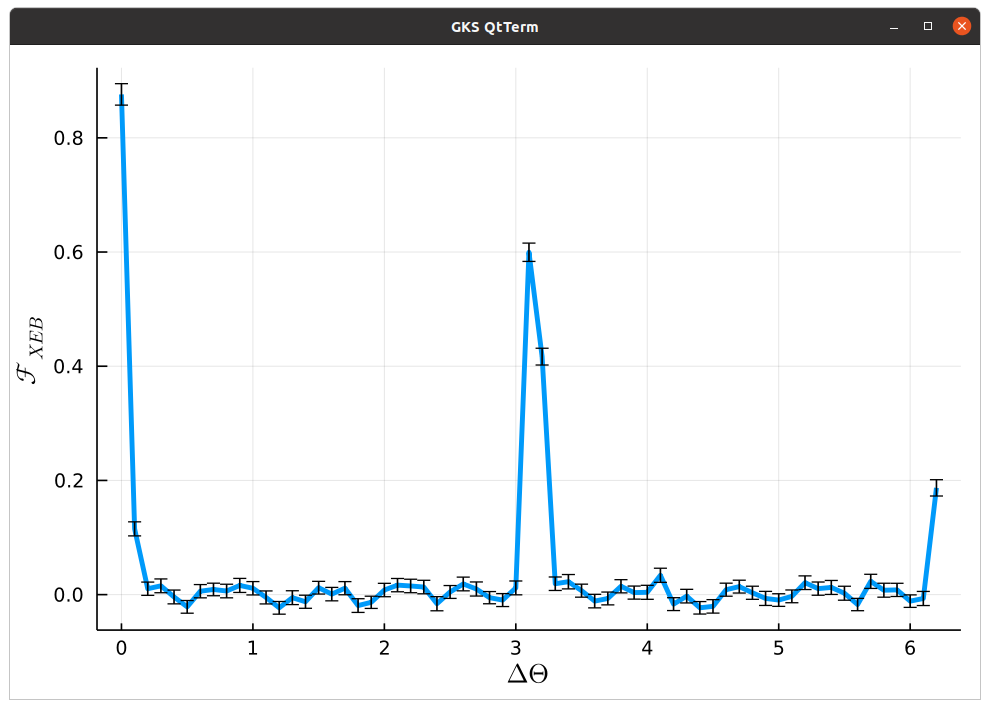
\includegraphics[width=\linewidth]
		{figures/Task4b_N_4_d_128_s_400}
		\subcaption{\label{fig:task4b_N4}}
	\end{subfigure}%b
	
	\begin{subfigure}[t]{0.42\textwidth}
		\centering
		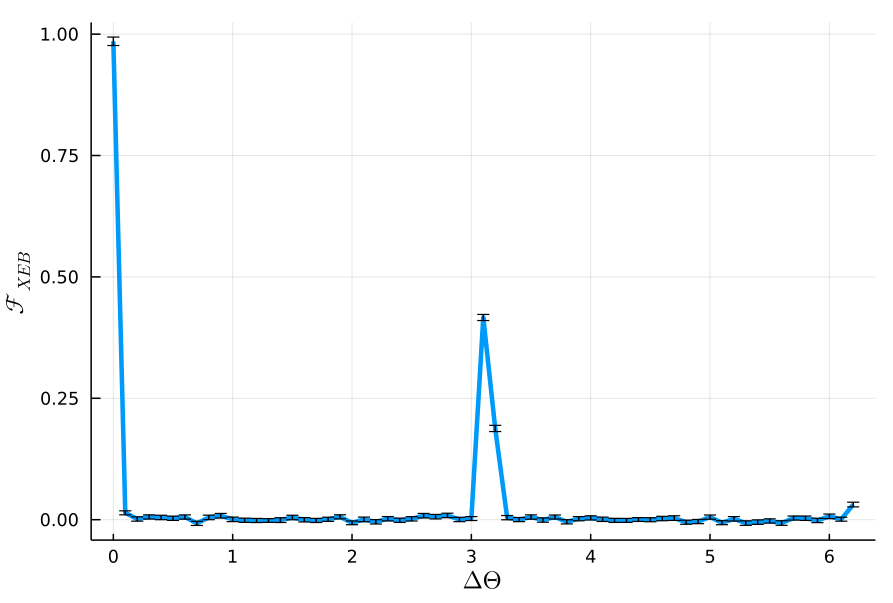
\includegraphics[width=\linewidth]
		{figures/Task4b_N_8_d_128_s_200}
		\subcaption{\label{fig:task4b_N8}}
	\end{subfigure}%c
	\begin{subfigure}[t]{0.42\textwidth}
		\centering
		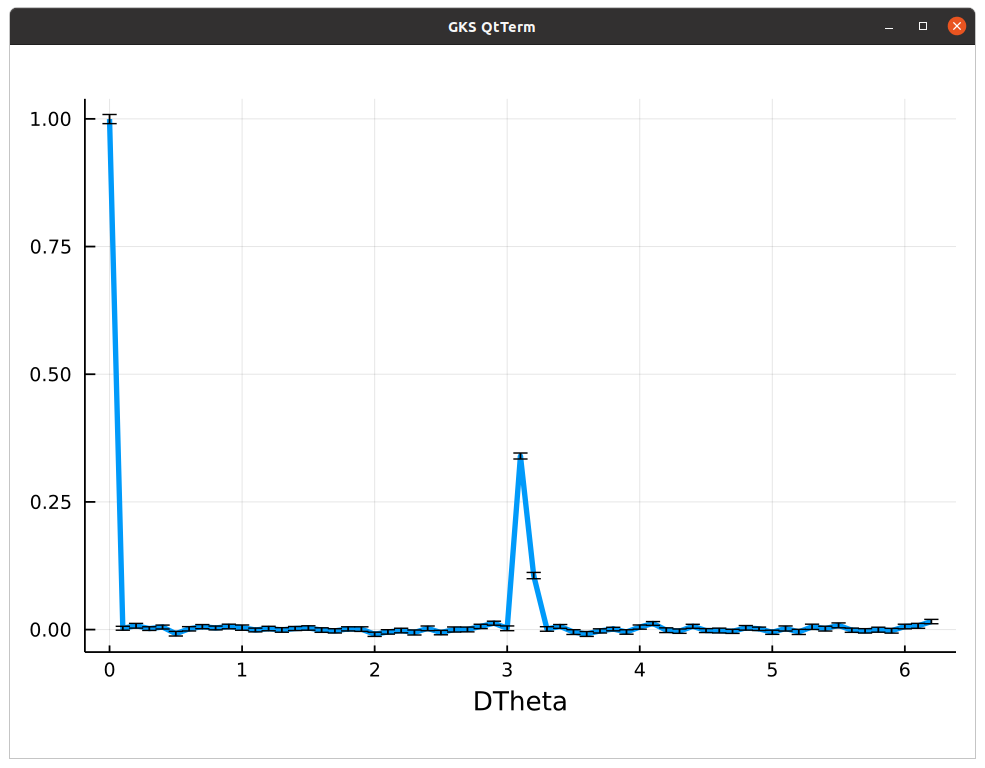
\includegraphics[width=\linewidth]
		{figures/Task4b_N_10_d_128_s_50_fg}
		\subcaption{\label{fig:task4b_N10}}
	\end{subfigure}%d
	\caption{
		The crossed entropy benchmarking fidelity $\mathcal{F}_\mathrm{XEB}$ calculated as a function of the perturbation angle $\Delta \Theta$ in a unit of radians at different numbers of qubit $N$, circuit depths $d$, and numbers of samples $s$. \subref{fig:task4} $N$=8, $d$=512, without averaging; \subref{fig:task4b_N4} $N$=4, $d$= 128, $s$=400; \subref{fig:task4b_N8} $N$=8, $d$=128, $s$=200; \subref{fig:task4b_N10} $N$=10, $d$=128, $s$=50.
	}
	\label{fig:XEBfidelity}
\end{figure}

\section*{Business Application}

We would like to apply this quantum advantage in the seismic signal processing for oil exploration business, which is one of the ten biggest Industries in the world and its annual market revenue would be around \$3 trillion USD \cite{oil_industry}. This would be particularly relevant for Canada as it is a national industry, being present in almost all provinces. 

As a widely applicable technique, seismic technologies are exploited in the development of oil and gas production by constructing subsurface images both in two- and three-dimensions \cite{subsurface_img, dug}. Thus, it is required to collect enormous big data and interpret them correctly and efficiently. 
Seismic modeling is an inherently noisy process as such most models and interpretations can tolerate noise inherently present in the data. This provides a unique avenue for NISQ devices where noise related fidelity is a concern. With further investigation we will be able to ascertain the degree to which NISQ can contribute. 
By trading noise for the efficiency, our team believes that powerful quantum machines will outperform classical computing performance to handle massive seismic wave data efficiently and to reach correct interpretations for timely business decisions with optimal performance and economical benefits. (Please refer to \href{https://youtu.be/qaflxbQGtgc}{\underline{https://youtu.be/qaflxbQGtgc}} for our video about the business application.)

\begin{thebibliography}{10}

\bibitem{oil_industry} \href{https://www.investopedia.com/investing/oil-gas-industry-overview/}{https://www.investopedia.com/investing/oil-gas-industry-overview/}
\bibitem{subsurface_img} \href{https://gov.nu.ca/sites/default/files/2017_seismic_eng.pdf}{https://gov.nu.ca/sites/default/files/2017\_seismic\_eng.pdf}
\bibitem{dug} \href{https://dug.com/dug-insight/}{https://dug.com/dug-insight/}

\end{thebibliography}

\end{document}
